\chapter{提案手法}

本章では、実験で用いる提案モデルとデータセットについて説明した後、実験結果の考察を行う。

\section{データセットと音の表現}

データセットとして1秒のギターとハープの音の88組を用いた。88音としてはA0$\sim$C8の半音を全て選び、これらは一般的な88鍵のピアノのそれぞれの鍵盤の音に対応する~(図\ref{fig:piano})~。また、ギターとハープを変換対象とした理由は、弦楽器という共通点を持ちながらも人間の耳で十分に異なると判定できる楽器であると考えられたからである。

そして、44100~Hzのサンプリング周波数でサンプリングを行い、音響信号を圧縮せずに保持するWAV形式によりデータを生成した。また、量子化ビット数は16ビット、チャンネル数は1である。したがって、本研究で用いる音は44100の長さを持つ16ビット整数の一次元配列として表現される。

\begin{figure}[b]
\begin{center}
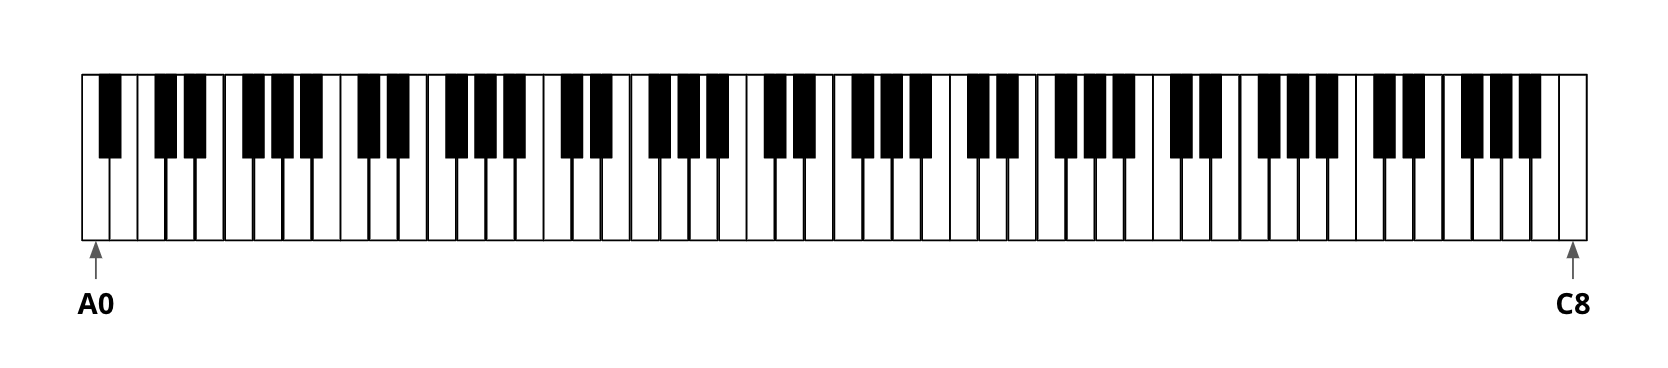
\includegraphics[width=0.9\hsize]{figure/piano.png}
\caption{88鍵のピアノの鍵盤}
\label{fig:piano}
\end{center}
\end{figure}

%ここで改ページ

\section{提案モデル}
\label{sec:proposed}

本研究では、Pix2pix~\cite{pix2pix}を元に生成モデルと識別のいずれにも条件として変換元の音を入力することで音色の変換を行うGANを提案モデルとして作成した~(図\ref{fig:pr_model})~。また、このモデルでは決定論的に音を生成するために生成モデルの入力にノイズを使用していない。

そして、本節の図の灰色の箱は複数のチャンネルを持つ特徴量マップである。箱の上側にチャンネル数を示し、箱の左側に特徴量マップとなる一次元配列の長さを示す。また、ネットワーク構造の下にそれぞれの矢印の操作の内容を示す。ConvolutionとDeconvolutionについては~(カーネルサイズ、パディング数、ストライド幅)~としてそれぞれの値を示し、LeakeyReLUについては負の実数の定義域での一次関数の傾きの値を示す。

\begin{figure}[t]
\begin{center}
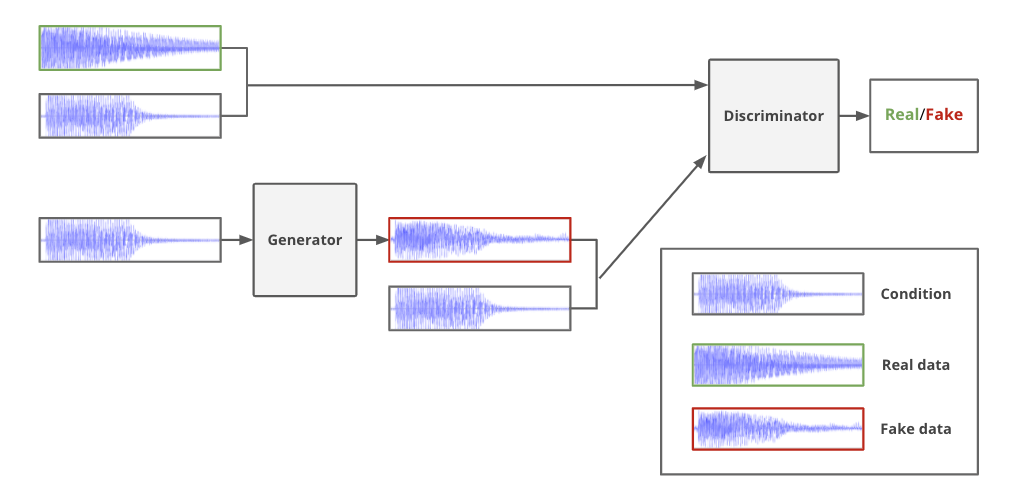
\includegraphics[width=0.8\hsize]{figure/pr_model.png}
\caption{提案モデル}
\label{fig:pr_model}
\end{center}
\end{figure}

\subsection{生成モデル}

生成モデルには1つのスキップコネクションを持つEncoder-Decoder型のネットワークを用いた。また、入力は条件となる変換元の音波である~(図\ref{fig:pr_gen})~。

\begin{figure}[b]
\begin{center}
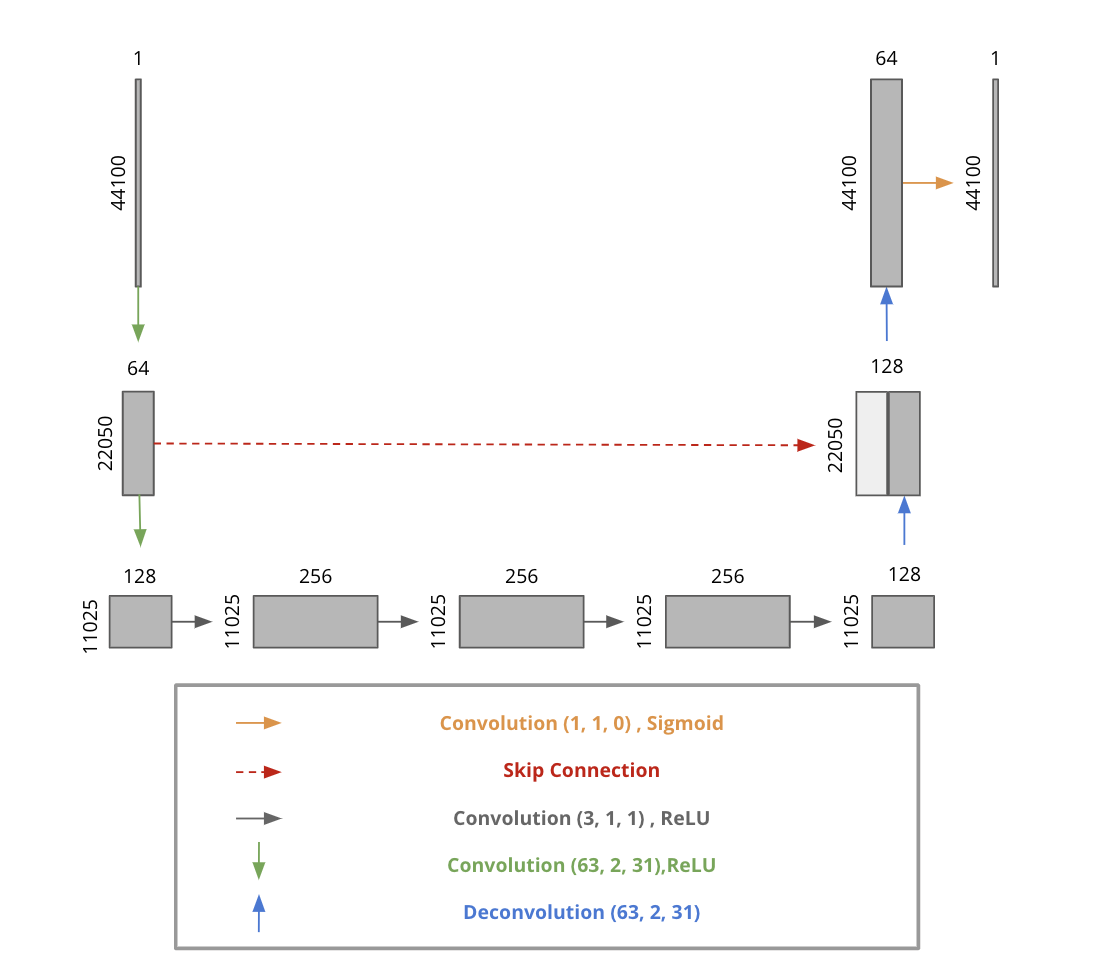
\includegraphics[width=0.6\hsize]{figure/pr_generator.png}
\caption{生成モデル\\
図は~\cite{u-net}のFigure~1を参考に作成した。}
\label{fig:pr_gen}
\end{center}
\end{figure}

%ここで改ページ

\subsection{識別モデル}

識別モデルには一般的なCNNを用いた。また、出力は最終層の特徴量マップの平均値である~(図\ref{fig:pr_dis})~。

\begin{figure}[b]
\begin{center}
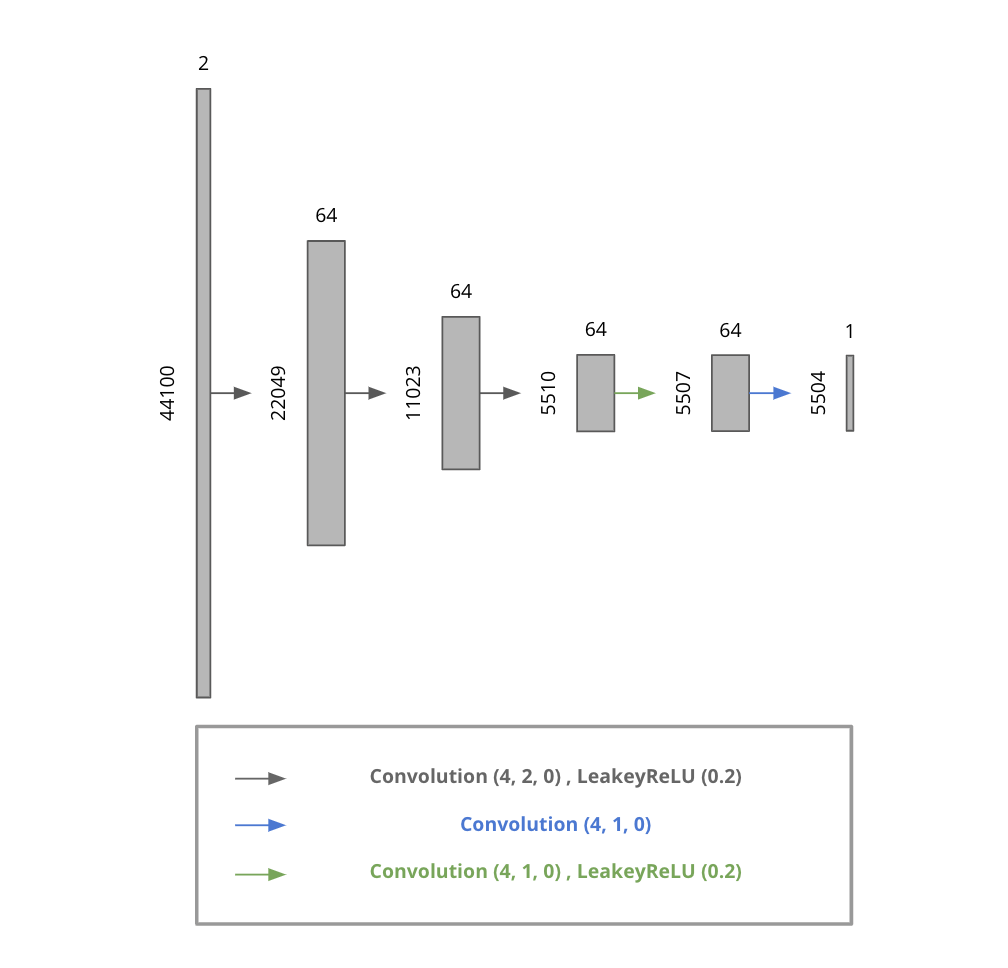
\includegraphics[width=0.6\hsize]{figure/pr_discriminator.png}
\caption{識別モデル\\
図は~\cite{u-net}のFigure~1を参考に作成した。}
\label{fig:pr_dis}
\end{center}
\end{figure}

\section{実験方法}

\ref{sec:proposed}節の提案モデルを用いてギターからハープへの単音の変換の実験を行った。学習の際の最適化アルゴリズムとしてはAdam~\cite{Adam}を用いた。また、学習時のパラメータは\ref{sec:appendix_params}節に示す。

\subsection{提案モデルの表現力の評価実験}

提案モデルの表現力を評価する実験を行った。具体的には、用意した88音を学習データと評価データのいずれでも使用し、同じ高さの音の間での変換の実験を行った。

\subsection{提案モデルの汎化能力の評価実験}

単色の音色変換であっても任意の高さと大きさの音を学習データとして用意するのは不可能であるため、提案モデルの汎化能力を評価する必要がある。ここでは、88音のうち3/4を学習データ、1/4を評価データとする4分割交差検定により実験を行った。また、データセットの分割方法は\ref{sec:appendix_split}節に示す。

\subsection{評価方法}

生成した音は音波の波形の観察と音の聴き取りにより評価した。また、生成モデルの出力が音の高さ及び音の大きさを保持したまま変換先のハープの音の音色に変換できているかという観点から評価を行った。

\subsection{データ拡張}

%位相をずらす、バッチサイズの調整?
各エポックの任意の学習データの振幅を無作為化することでデータ拡張を行った。具体的には、学習前に乱数のシードを固定した後に一様乱数により$0.3\sim1.0$の乱数を生成した。また、これにより88音と小さいサイズのデータセットへの過学習を防ぐことを期待した。

%ここで改ページ

\section{実験結果}
%ここを改変、楽音→音の高さ→音の音色で達成度をまずは書く

本節では、実験結果とその考察をまとめる。また、実験結果に記載する波形の図は三つの波形を上から並べている。これらは上から順に、変換元のギターの波形、生成モデルの出力波形、変換先のハープの波形、である。

\subsection{生成モデルの表現力の評価実験}
\label{sec:expression}
%lossの図

\begin{figure}[b]
\begin{center}
\begin{minipage}{0.48\hsize}
\begin{center}
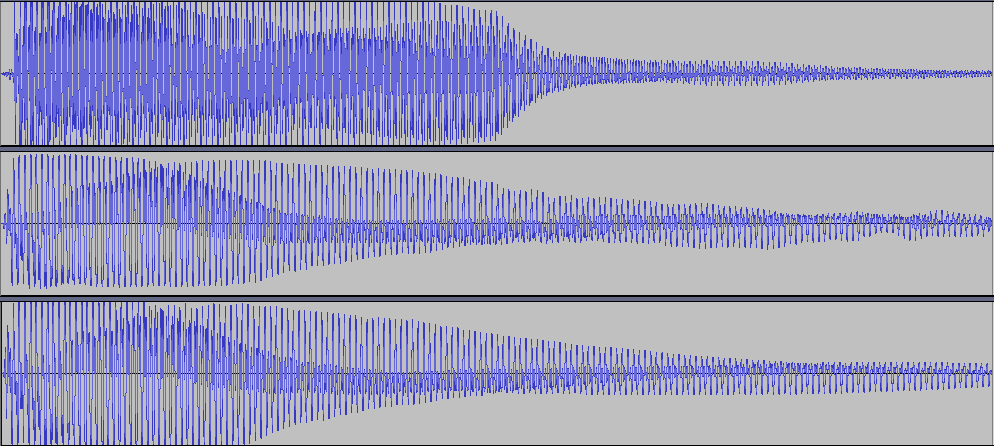
\includegraphics[width=0.9\hsize]{figure/88_88/f3.png}
\caption{F3の0.800秒から1.000秒までの音波}
\label{fig:88_88_good1}
\end{center}
\end{minipage}
\begin{minipage}{0.48\hsize}
\begin{center}
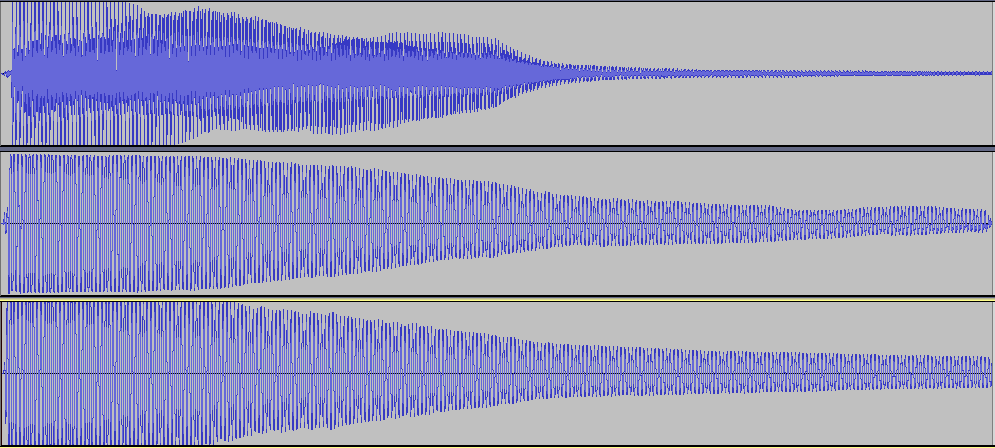
\includegraphics[width=0.9\hsize]{figure/88_88/c4.png}
\caption{C4の0.200秒から0.300秒までの音波}
\label{fig:88_88_good2}
\end{center}
\end{minipage}
\end{center}
\end{figure}


まず、F2からG6$\sharp$の音は耳で聴いても波形を見ても図\ref{fig:88_88_good1}のように正確にハープの音を表現することができていた。特にC4からD5$\sharp$の音は図\ref{fig:88_88_good2}のように上音の音が少ないために綺麗なハープの音を生成することができていた。他の音についても下記に挙げた改善点はあるものの基音の部分は表現することができていた。以下では、ハープの音を生成において困難であった点を列挙する。


\subsubsection{音波の振幅}

\begin{figure}[t]
\begin{center}
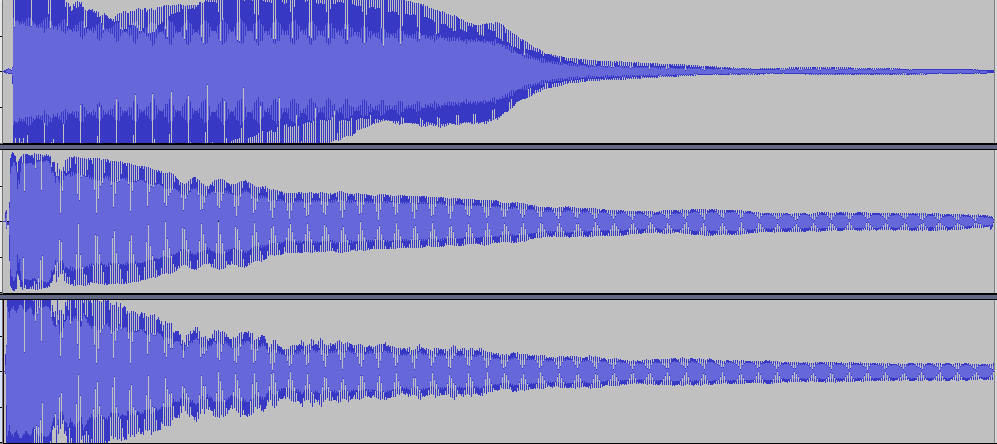
\includegraphics[width=0.7\hsize]{figure/88_88/c5.png}
\caption{C5の0.000秒から1.000秒までの音波}
\label{fig:88_88_amp}
\end{center}
\end{figure}

図\ref{fig:88_88_amp}の波形の前半のように、生成された波形の振幅が小さいという問題が発生した。これにより、減衰していく部分の表現が難しい場合があった。原因は、振幅をランダムに小さくしたためであると考えられ、学習の初段階では振幅を固定するなどの工夫する必要があると思われる。
    
\subsubsection{音の鳴り出しの遅延}

\begin{figure}[t]
\begin{center}
\begin{minipage}{0.48\hsize}
\begin{center}
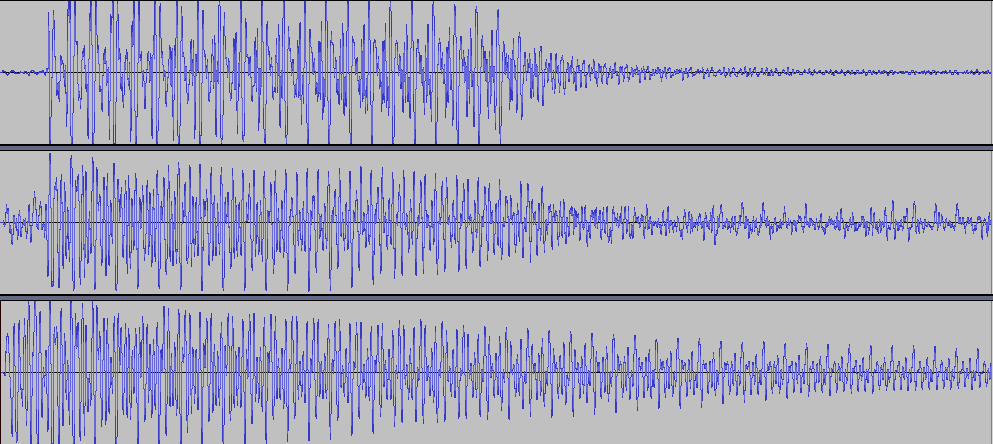
\includegraphics[width=0.9\hsize]{figure/88_88/f1s.png}
\caption{F1$\sharp$の0.000秒から1.000秒までの音波}
\label{fig:88_88_lag1}
\end{center}
\end{minipage}
\begin{minipage}{0.48\hsize}
\begin{center}
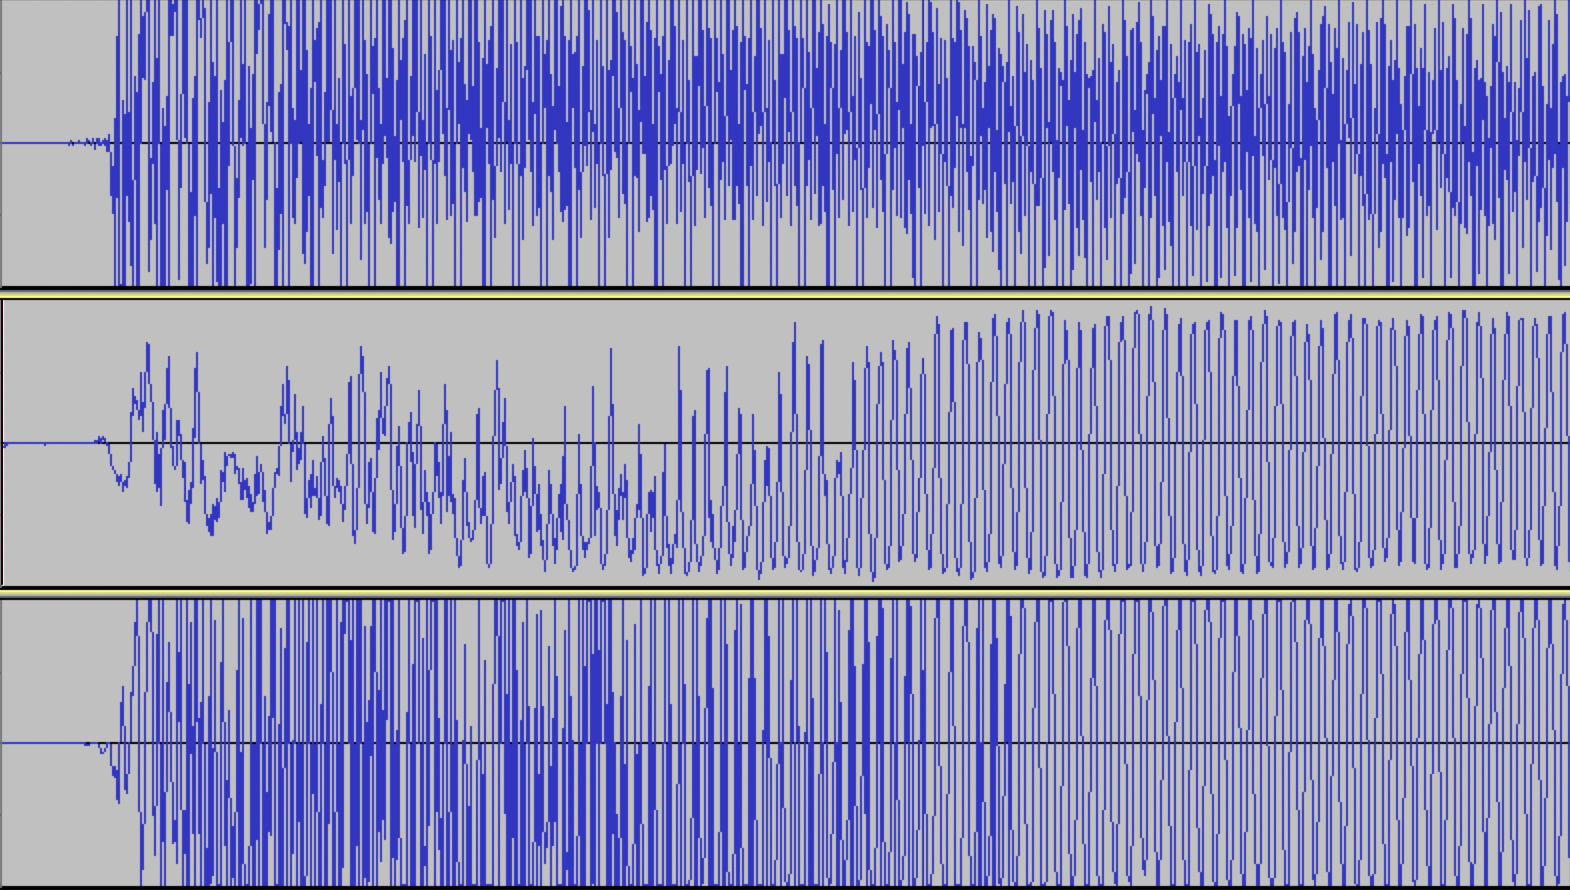
\includegraphics[width=0.9\hsize]{figure/88_88_det/a7_0_0030.png}
\caption{A7の0.000秒から0.030秒までの音波}
\label{fig:88_88_lag2}
\end{center}
\end{minipage}
\end{center}
\end{figure}

ギターとハープは弦楽器なので鳴り出すまでに遅延がある。特に、今回用いたデータセットでは図\ref{fig:88_88_lag1}のようにギターの音に遅延がある場合や図\ref{fig:88_88_lag2}のように周期的な音になるまでに遅延がある場合、その部分を学習することが難しかった。

\subsubsection{音波の滑らかさ}

\begin{figure}[t]
\begin{center}
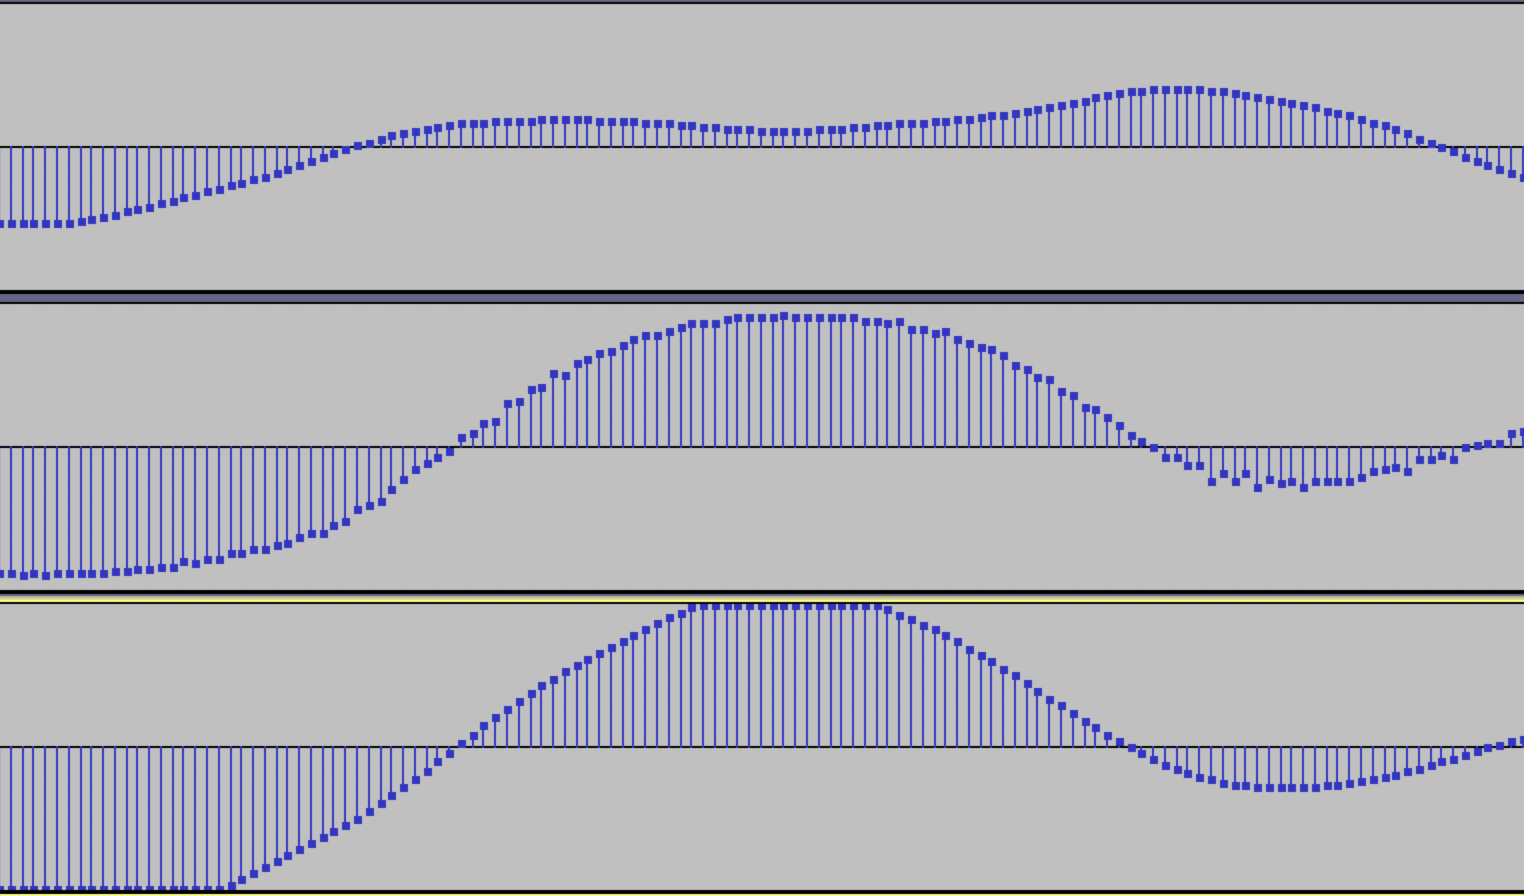
\includegraphics[width=0.7\hsize]{figure/88_88_det/d2s_0100_0103.png}
\caption{D2$\sharp$の0.100秒から0.103秒までの音波}
\label{fig:88_88_smooth}
\end{center}
\end{figure}

%滑らかさの表現
図\ref{fig:88_88_smooth}の上から2番目の波形と3番目の波形を比較すると、生成された波には滑らかさがないことがわかる。人間の耳にはこの滑らかでない音波の部分はノイズまじりの音として聞こえるので、この波を滑らかにするための工夫が必要であると考えられる。

\subsubsection{音波の振動の減衰}

\begin{figure}[t]
\begin{center}
\begin{minipage}{0.48\hsize}
\begin{center}
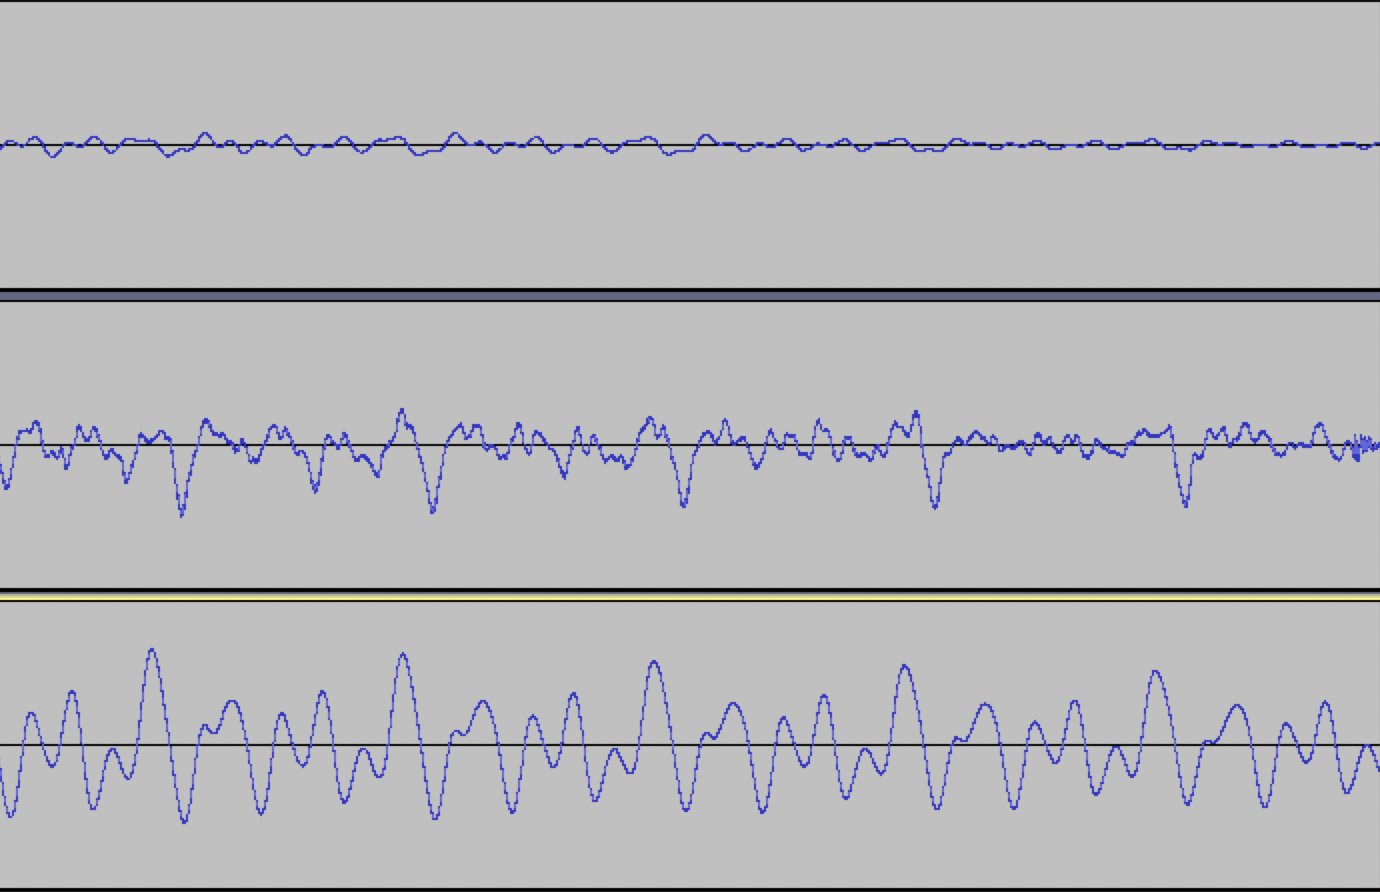
\includegraphics[width=0.9\hsize]{figure/88_88_det/a0_0800_1000.png}
\caption{A0の0.800秒から1.000秒までの音波}
\label{fig:88_88_reduce1}
\end{center}
\end{minipage}
\begin{minipage}{0.48\hsize}
\begin{center}
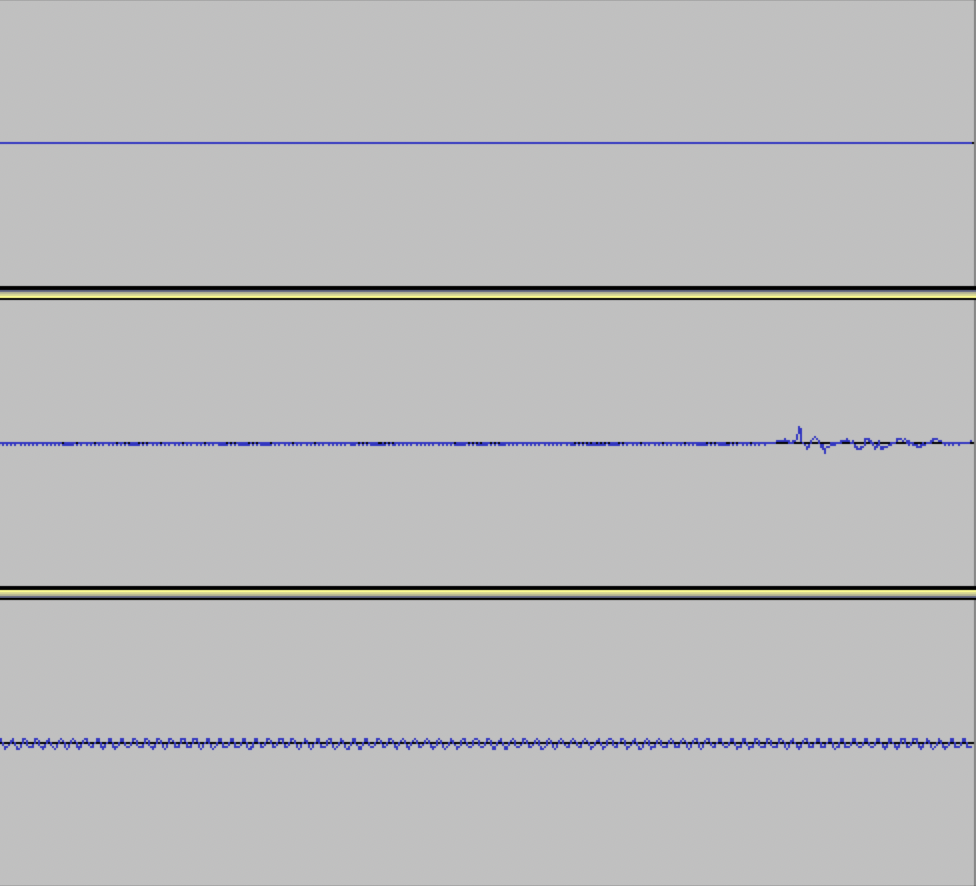
\includegraphics[width=0.9\hsize]{figure/88_88_det/b7_0980_1000.png}
\caption{B7の0.980秒から1.000秒までの音波}
\label{fig:88_88_reduce2}
\end{center}
\end{minipage}
\end{center}
\end{figure}

音波の振動の減衰が全く表現できていない音波があった。具体的には、A0,A0$\sharp$,B0,C1,C1$\sharp$,D1,D1$\sharp$,E1,\\
F1,F1$\sharp$,G1,G1$\sharp$D2,D2$\sharp$,E2,A6,A6$\sharp$,B6,C7,C7$\sharp$,D7,D7$\sharp$,F7,F7$\sharp$,G7,G7$\sharp$,A7,A7$\sharp$,B7,C8の音である。また、これ以外の音についても減衰が一部表現できていないものはあった。

これらの音のうち、E2以下の低音域の場合は図\ref{fig:88_88_reduce1}のようにハープとは全く異なる波形で減衰し、A6以上の高音域の場合は図\ref{fig:88_88_reduce2}のようにほとんど振動が見られなかった。原因としては、微小な振動をニューラルネットワークが学習するのが難しいことと今回のデータセットではギターの方がハープよりも音の鳴る時間が短かったことが挙げられる。

\subsubsection{安定したデータセットの作成}

\begin{figure}[t]
\begin{center}
\begin{minipage}{0.48\hsize}
\begin{center}
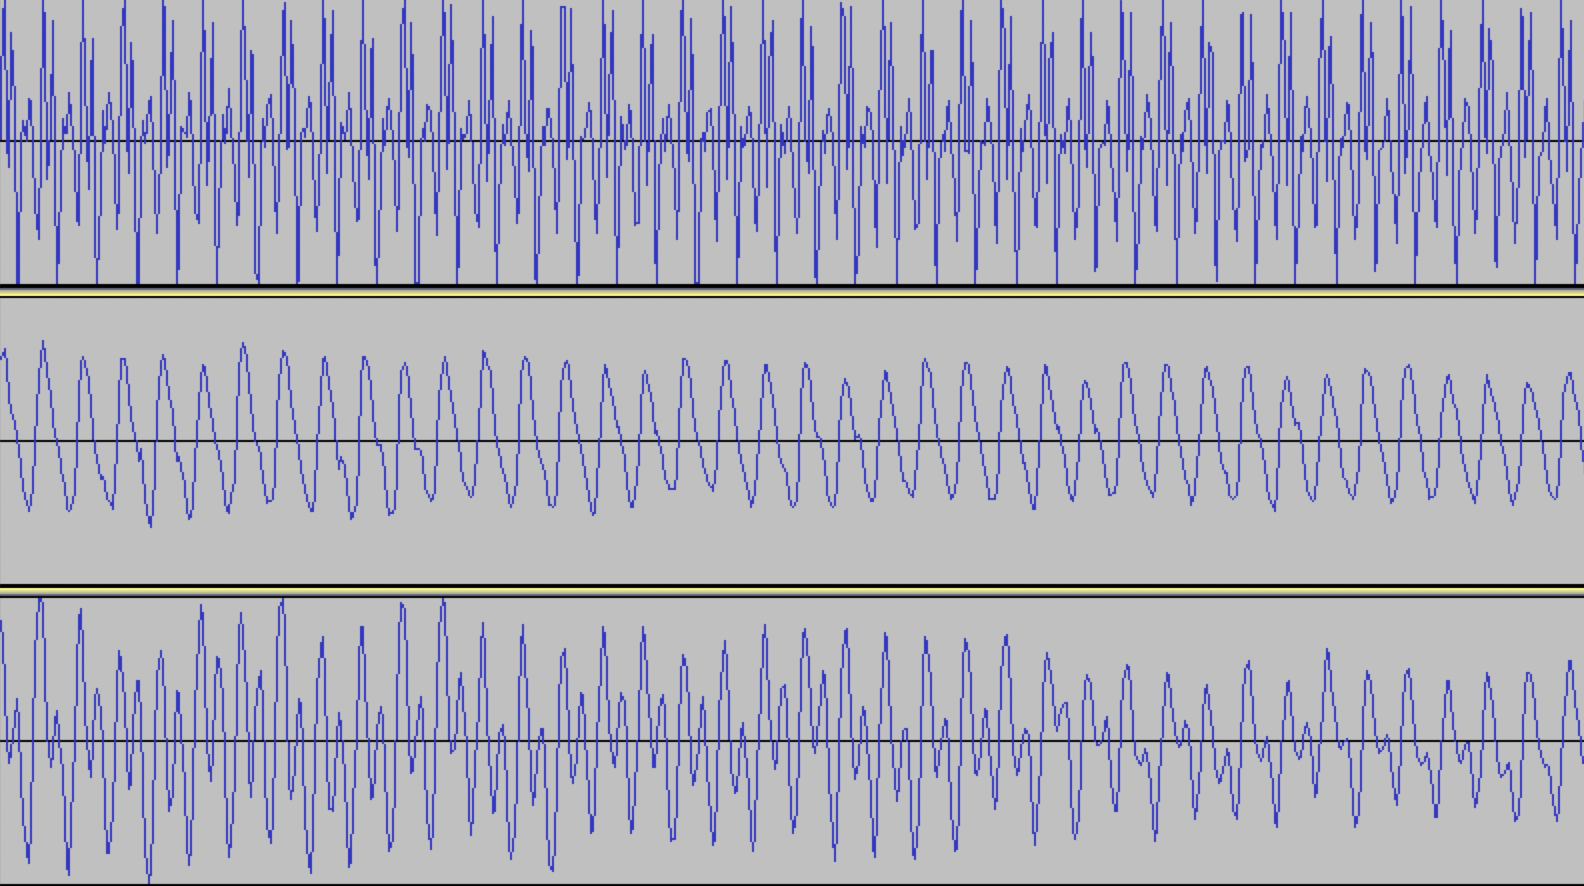
\includegraphics[width=0.9\hsize]{figure/88_88_det/e7_0550_0700.png}
\caption{E7の0.055秒から0.070秒までの音波}
\label{fig:88_88_bad1}
\end{center}
\end{minipage}
\begin{minipage}{0.48\hsize}
\begin{center}
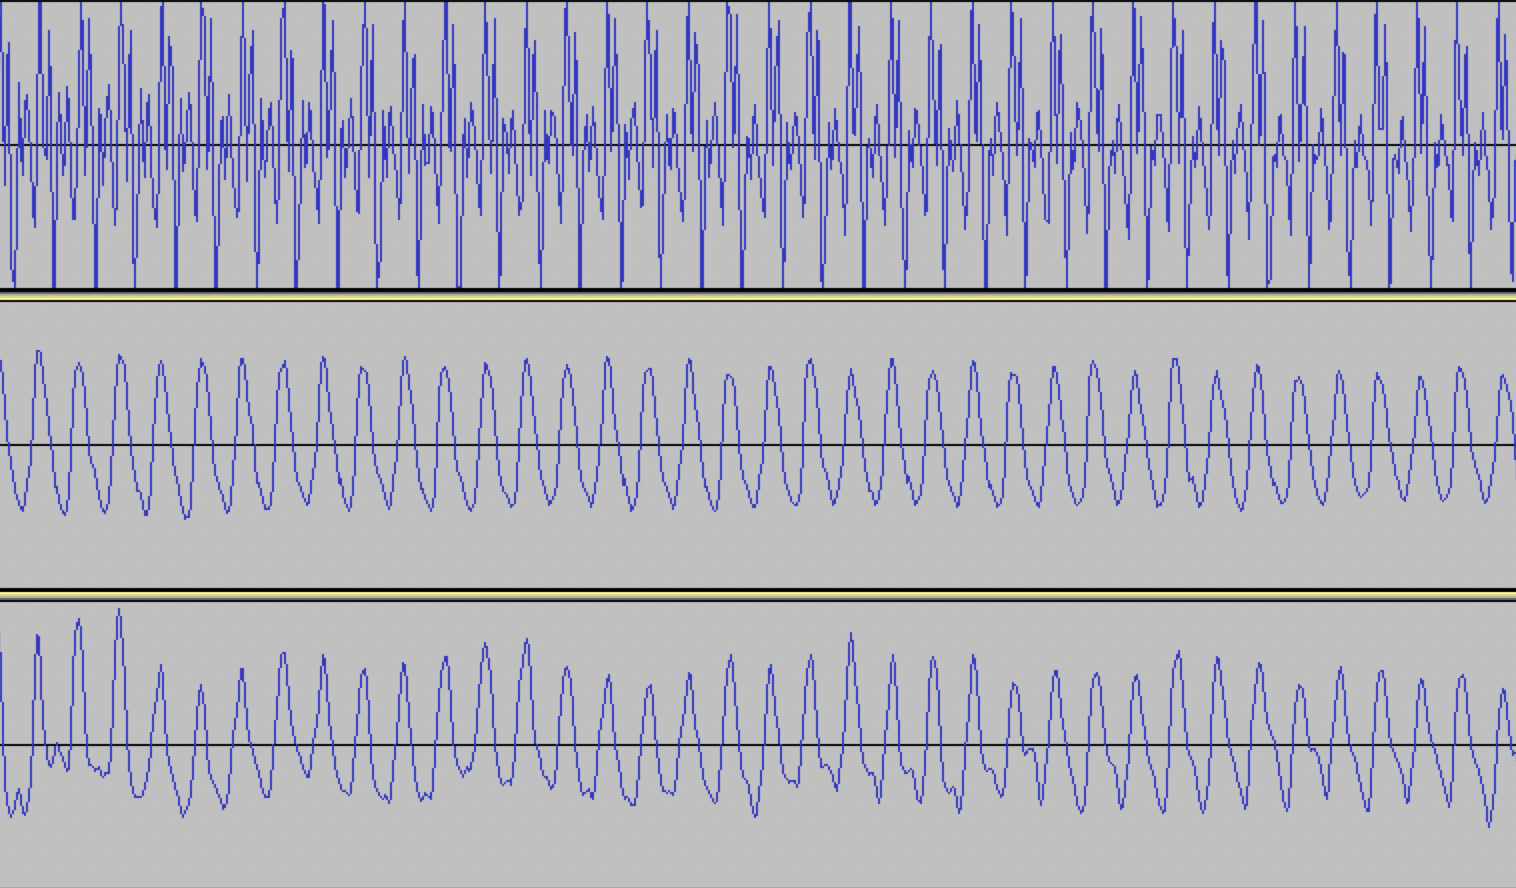
\includegraphics[width=0.9\hsize]{figure/88_88_det/d7s_0550_0700.png}
\caption{D7$\sharp$の0.055秒から0.070秒までの音波}
\label{fig:88_88_bad2}
\end{center}
\end{minipage}
\end{center}
\end{figure}

E7の音については、図\ref{fig:88_88_bad1}のように上記に挙げた以外の部分で波が表現できていなかったが、ハープのデータセットの音波の振動の振幅が安定していないために、ニューラルネットワークによる学習が難しかったと考えられる。

また、E7の半音下の音であるD7$\sharp$でも図\ref{fig:88_88_bad2}のようにハープのデータセットの音波の振動の振幅は安定しておらず、特に高音は安定した振幅のデータセットを生成することが難しいと考えられる。

\subsection{生成モデルの汎化能力の評価実験}

まず、音の高さは変換前後で変わってないものが多く期待通りの結果となった。しかし、音の音色は元のギターの音色とは異なるもののハープとも異なる音色となり、\ref{sec:expression}節における課題も解決することはできなかった。以下では、生成されたハープの音について波形を元に考察を行う。

%学習の際のlossの図

\subsubsection{音波の単純さ}

\begin{figure}[t]
\begin{center}
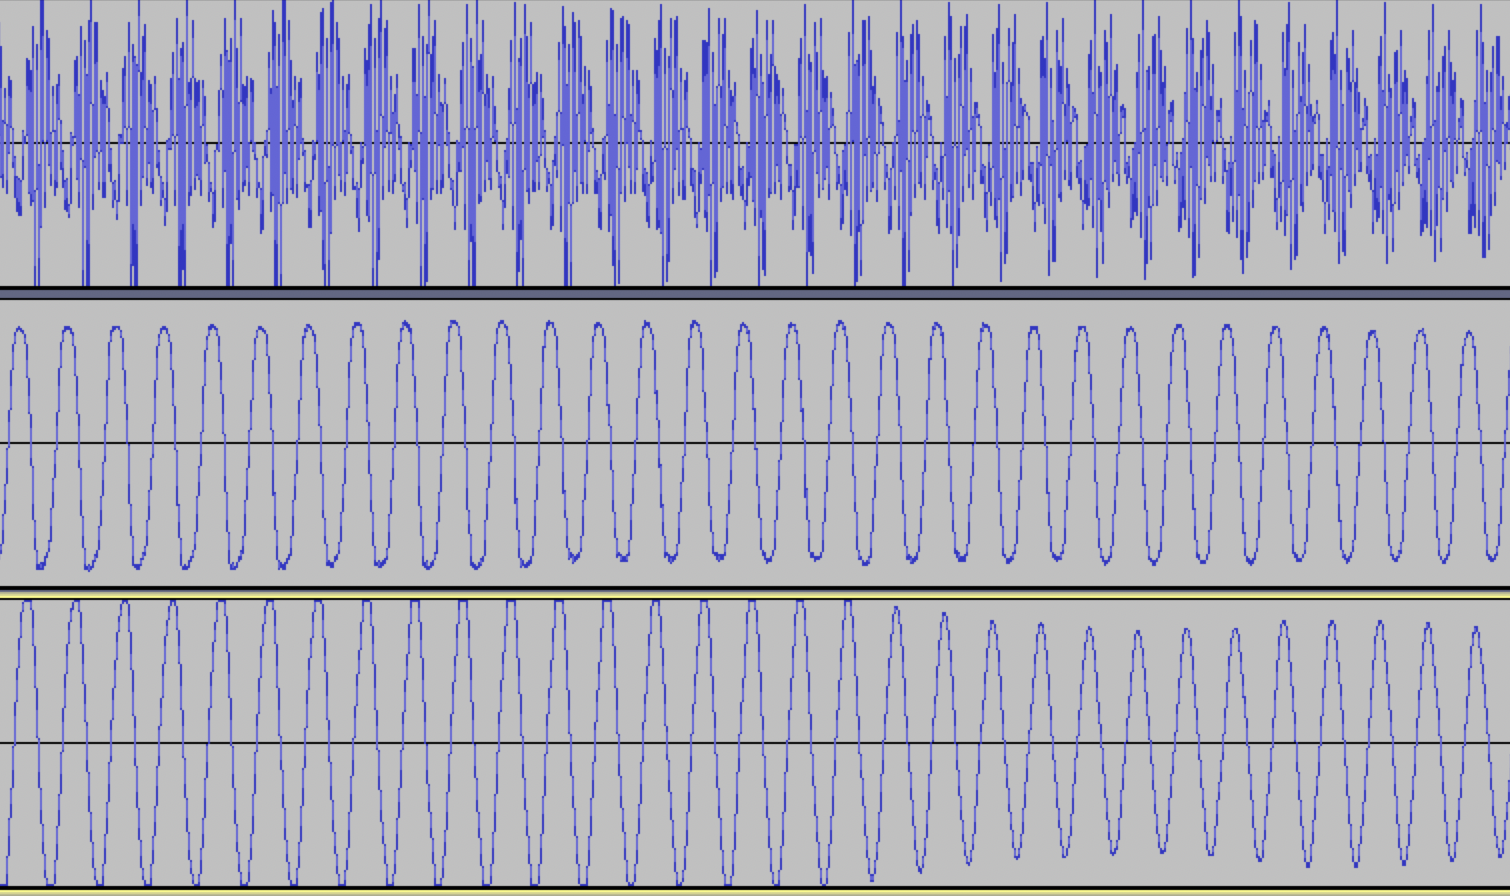
\includegraphics[width=0.7\hsize]{figure/66_22_det/d4s_0100_0200.png}
\caption{D4$\sharp$の0.100秒から0.200秒までの音波}
\label{fig:66_22_near}
\end{center}
\end{figure}

\ref{sec:expression}節と同程度にハープに近い音が生成される場合もあった。具体的には、D4,D4$\sharp$,G4,F5,F5$\sharp$の音である。これらの音は、音波が図\ref{fig:66_22_near}のように単純な波形でニューラルネットワークによる表現が容易であるため、生成が他の音波に比べて容易であったと考えられる。

\subsubsection{音波の複雑さ}

\begin{figure}[t]
\begin{center}
\begin{minipage}{0.48\hsize}
\begin{center}
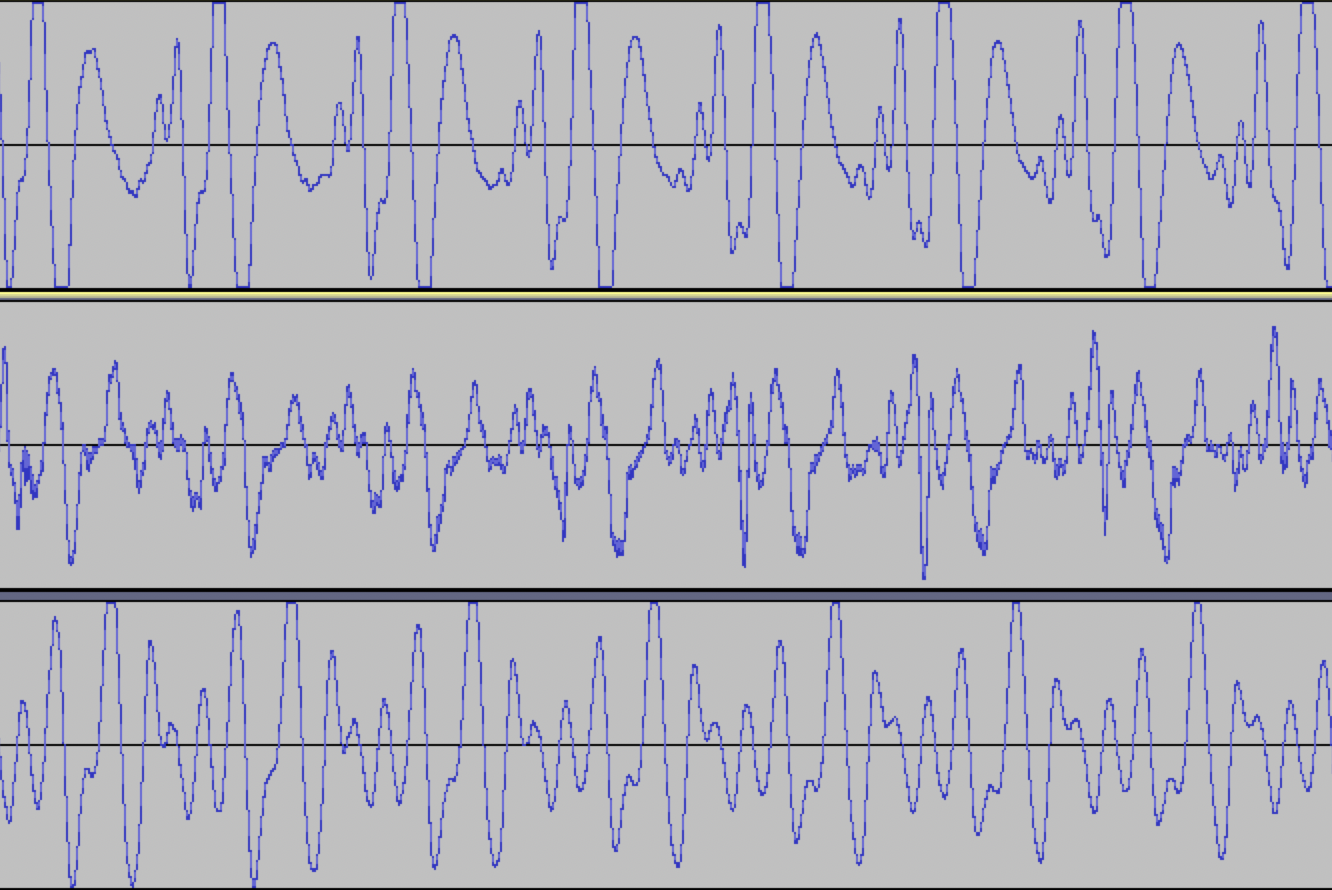
\includegraphics[width=0.9\hsize]{figure/66_22_det/d1_0300_0500.png}
\caption{D1の0.300秒から0.500秒までの音波}
\label{fig:66_22_bad1}
\end{center}
\end{minipage}
\begin{minipage}{0.48\hsize}
\begin{center}
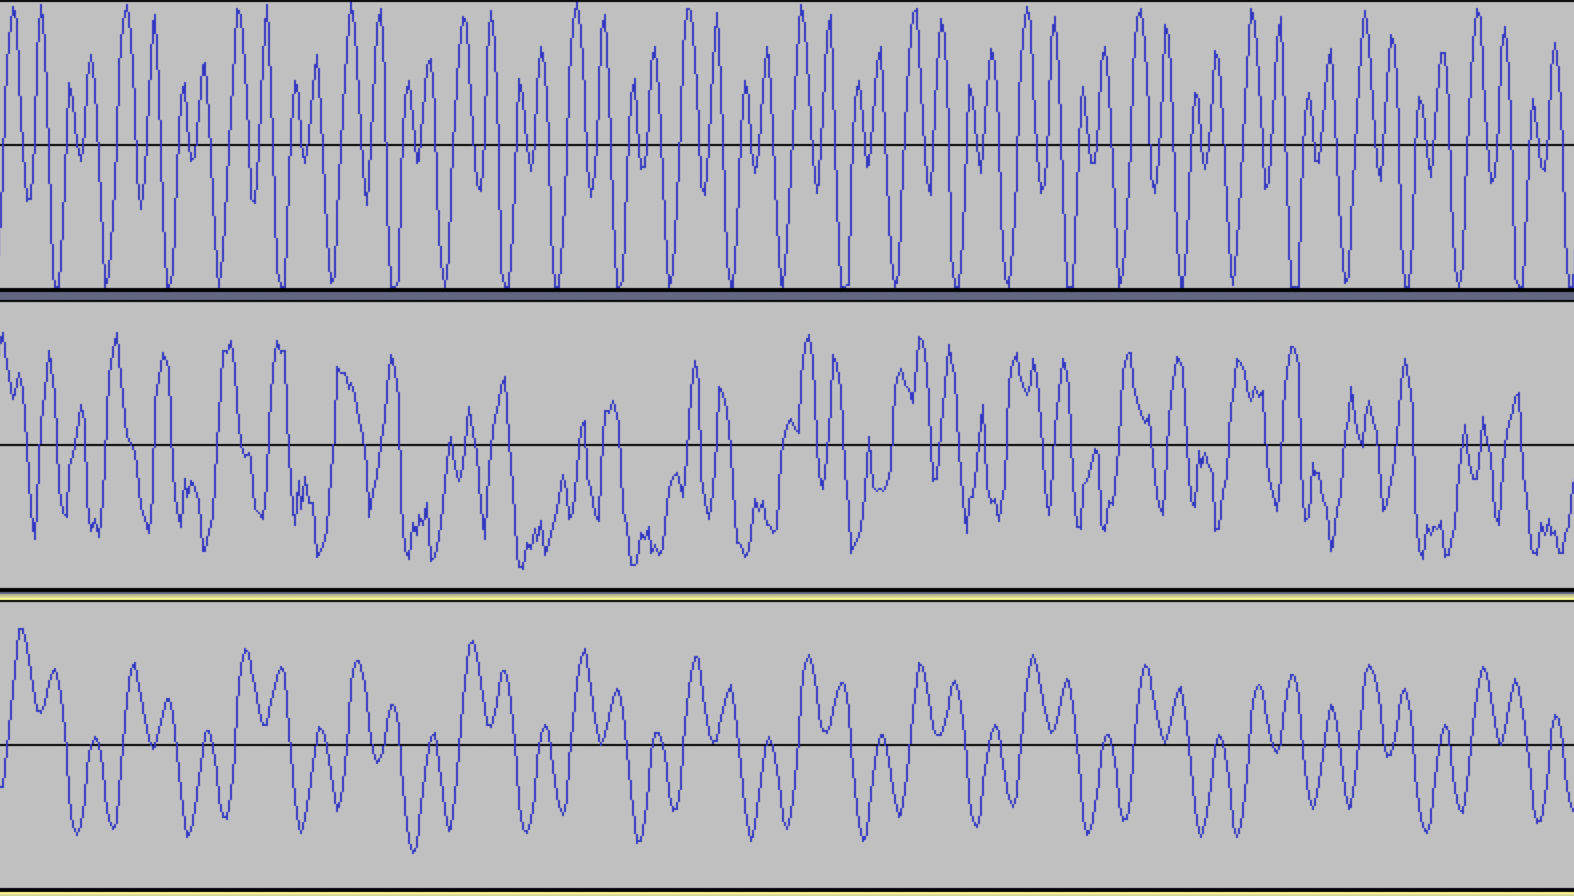
\includegraphics[width=0.9\hsize]{figure/66_22_det/f6_0070_0080.png}
\caption{F6の0.070秒から0.080秒までの音波}
\label{fig:66_22_bad2}
\end{center}
\end{minipage}
\end{center}
\end{figure}

\begin{figure}[t]
\begin{center}
\begin{minipage}{0.48\hsize}
\begin{center}
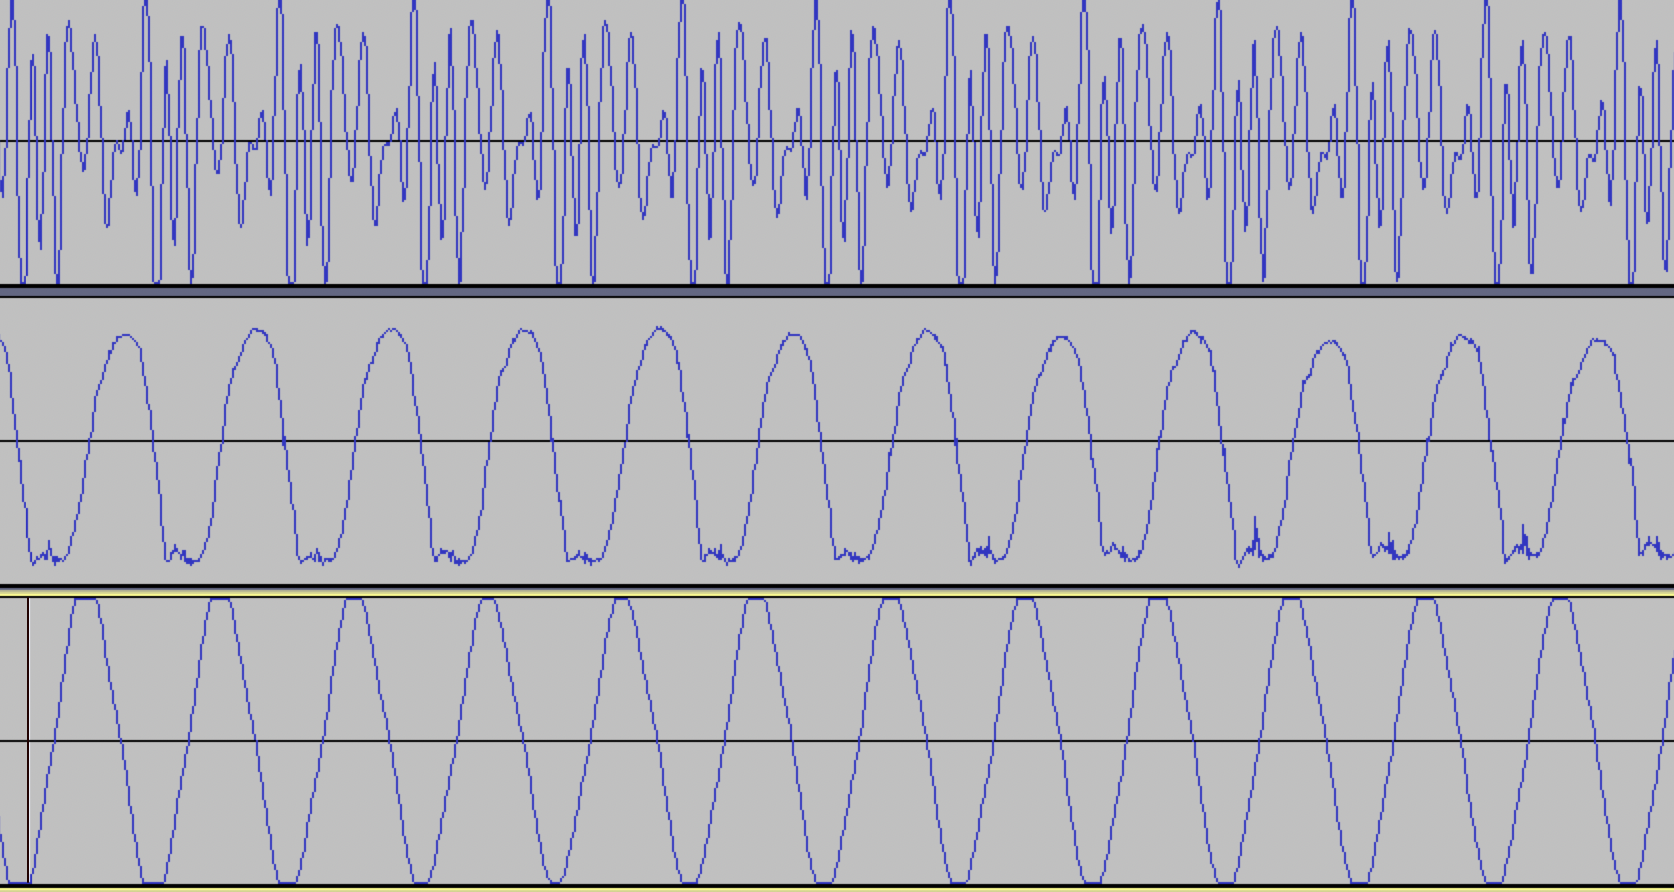
\includegraphics[width=0.9\hsize]{figure/66_22_det/g4s_0150_0180.png}
\caption{G4$\sharp$の0.150秒から0.180秒までの音波}
\label{fig:66_22_bad3}
\end{center}
\end{minipage}
\begin{minipage}{0.48\hsize}
\begin{center}
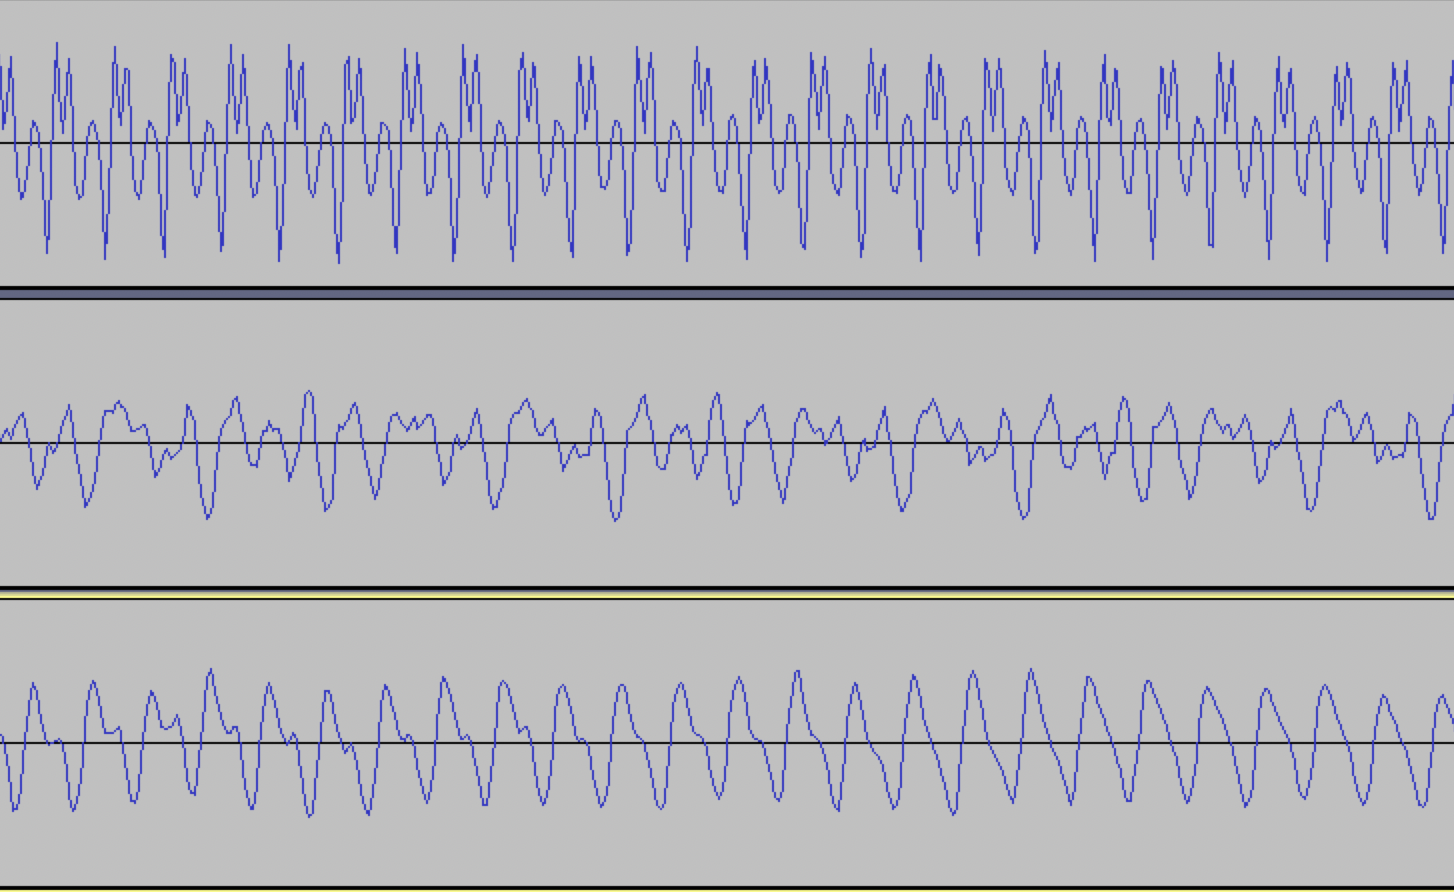
\includegraphics[width=0.9\hsize]{figure/66_22_det/d7s_0100_0110.png}
\caption{D7$\sharp$の0.1700秒から0.110秒までの音波}
\label{fig:66_22_bad4}
\end{center}
\end{minipage}
\end{center}
\end{figure}

上記の単純な音波以外の場合はギターの音色とは異なるもののハープの音色とも異なる音が生成された。いくつか種類があったが、図\ref{fig:66_22_bad1}や図\ref{fig:66_22_bad2}のように、音波が安定した振動をせず上音の成分がハープよりも多い音波が多く観測された。

また、ほとんどの音波において基音は保たれていたが、図\ref{fig:66_22_bad3}のように基音が同じで位相が異なる音波や図\ref{fig:66_22_bad4}のように基音が異なる音波が生成されることもあった。

これらの原因は、振幅をランダムにすることにより学習が安定しないことと微細な振動を表現可能なニューラルネットワークを構築できていないためと考えられる。後者の場合は画像で用いられるGANでの画像の高解像度化の工夫が適用できると期待される。